\chapter{Acid--Base Equilibria and the Predominant-Reaction Method}\label{ch:b1:predominant-reaction}

Vinegar dissolves the limescale of a kettle; so does lemon juice, a little
faster. Blood keeps its pH between narrow limits whatever we eat; a
fizzy drink is acidic because of the carbon dioxide dissolved in it. All
these are acid--base equilibria in water, and a chemist faced with a
solution containing several acids and bases --- a mixture, a buffer, a
\omterm{def:b1:predominant-reaction:polyprotic}{polyprotic acid} --- needs a reliable way to find its pH and the
concentrations of its species. This chapter builds that method: a scale of
strengths, diagrams of predominance, and the \emph{predominant-reaction
method}, which reduces any mixture to the one reaction that matters.

\begin{recall}
Book 1 (grade 12) defined \omterm{def:b1:predominant-reaction:bronsted}{Brønsted acids} and bases, the \omterm{def:b1:predominant-reaction:acidity-constant}{acidity constant}
$K_a$ and $\mathrm{p}K_a$, the \omterm{def:b1:predominant-reaction:autoprotolysis}{ionic product of water} and the pH of \omterm{def:b1:predominant-reaction:strong-acid}{strong
acids} and bases, and drew \omterm{def:b1:predominant-reaction:predominance}{predominance diagrams}. The \omterm{def:b1:extent-q-and-k:quotient}{reaction quotient},
the equilibrium constant and the activities of solutes ($c/c^\circ$) and
of the solvent (1) were defined in \cref{ch:b1:extent-q-and-k}; in this
chapter $c^\circ = \qty{1}{mol/L}$ is not written in quotients.
\end{recall}

\begin{omfigure}
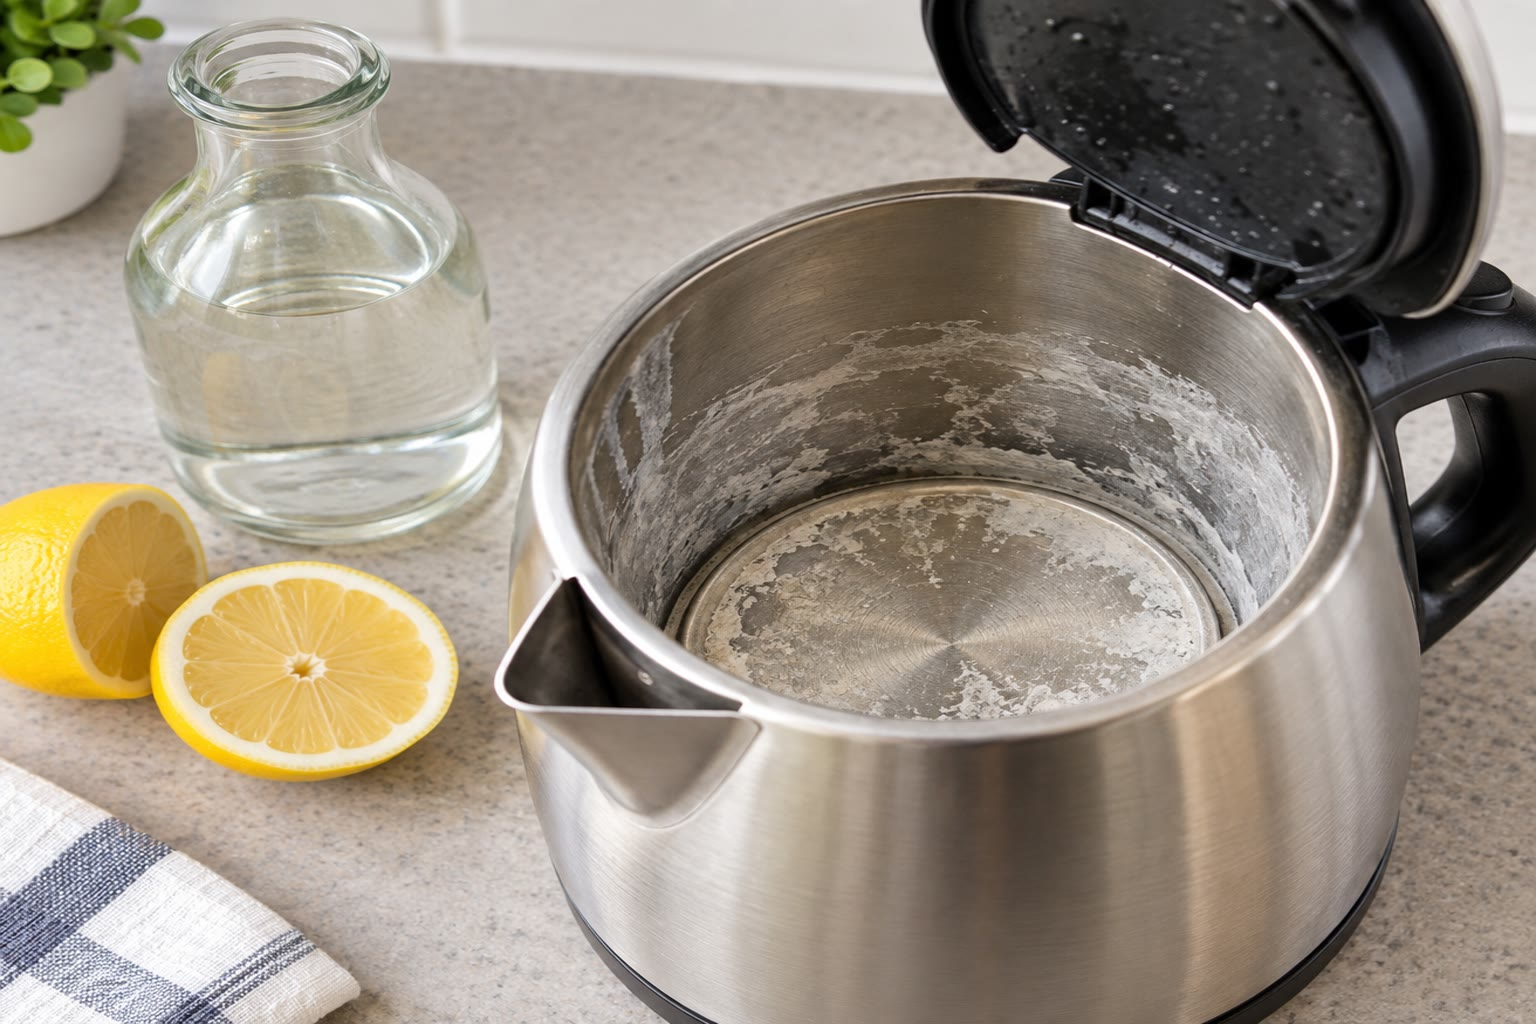
\includegraphics[width=0.5\linewidth]{images/book2/ai/b1-10-descaling.jpg}

{\small Limescale, calcium carbonate, in a kettle. The \omterm{def:b1:predominant-reaction:strong-acid}{weak acids} of
vinegar and lemon juice react with the carbonate ion and dissolve it.}
\end{omfigure}

\section{Brønsted couples and the pH}

\begin{definition}[Brønsted acid and base, couple]\label{def:b1:predominant-reaction:bronsted}
A \emph{Brønsted acid}\index{Brønsted acid} is a species able to give a
proton \ce{H+}; a \emph{Brønsted base}\index{Brønsted base} is a species
able to accept one. An acid HA and the base A that it becomes by losing a
proton form an \emph{acid--base couple}\index{acid--base couple} HA/A,
related by the formal half-equation $\mathrm{HA} \rightleftharpoons
\mathrm{A} + \ce{H+}$. In water the proton is never free: it is carried
by a water molecule as \ce{H3O+}.
\end{definition}

\begin{definition}[Ampholyte]\label{def:b1:predominant-reaction:ampholyte}
An \emph{ampholyte}\index{ampholyte} (an amphoteric species) is the base
of one couple and the acid of another: water (\ce{H3O+}/\ce{H2O} and
\ce{H2O}/\ce{OH-}), the hydrogencarbonate ion (\ce{CO2,H2O}/\ce{HCO3-}
and \ce{HCO3-}/\ce{CO3^{2-}}), the dihydrogenphosphate ion.
\end{definition}

\begin{definition}[Autoprotolysis, ionic product, pH]\label{def:b1:predominant-reaction:autoprotolysis}
Water undergoes \emph{autoprotolysis}\index{autoprotolysis},
\ce{2H2O <=> H3O+ + OH-}, of constant $K_e = [\ce{H3O+}][\ce{OH-}]$, the
\emph{ionic product of water}\index{ionic product of water}; at
\qty{25}{\celsius}, $K_e = 10^{-14.00}$, so $\mathrm{p}K_e = 14.00$. The pH
of a solution is $\mathrm{pH} = -\log a(\ce{H3O+}) \approx -\log[\ce{H3O+}]$.
A solution is neutral when $[\ce{H3O+}] = [\ce{OH-}]$, that is at
$\mathrm{pH} = \mathrm{p}K_e/2 = 7.00$ at \qty{25}{\celsius}.
% ledger: dfg:H2O_l, dfg:OH-_ao (pKe computed in figdata/bachelor-1/aqueous-constants.py)
\end{definition}

\section{Strength: \texorpdfstring{$K_a$}{Ka}, \texorpdfstring{p$K_a$}{pKa} and the levelling effect}

\begin{definition}[Acidity constant]\label{def:b1:predominant-reaction:acidity-constant}
The \emph{acidity constant}\index{acidity constant} of a couple HA/A is
the constant of the reaction of the acid with water,
\[
  \mathrm{HA} + \ce{H2O} \rightleftharpoons \mathrm{A} + \ce{H3O+}, \qquad
  K_a = \frac{[\mathrm{A}][\ce{H3O+}]}{[\mathrm{HA}]}, \qquad
  \mathrm{p}K_a = -\log K_a .
\]
The larger $K_a$ (the smaller $\mathrm{p}K_a$), the stronger the acid and
the weaker its conjugate base.
\end{definition}

\begin{definition}[Strong and weak acids and bases]\label{def:b1:predominant-reaction:strong-acid}
An acid is \emph{strong}\index{strong acid} in water if its reaction with
water is total: no molecule HA remains (hydrochloric, nitric, perchloric
acids, the first acidity of sulfuric acid); otherwise it is
\emph{weak}\index{weak acid}. A base is \emph{strong}\index{strong base}
if its reaction with water is total, giving \ce{OH-} (hydroxides, the
oxide ion, alkoxides), and \emph{weak}\index{weak base} otherwise.
\end{definition}

\begin{definition}[Levelling effect]\label{def:b1:predominant-reaction:levelling}
In water, every acid stronger than \ce{H3O+} reacts totally to give
\ce{H3O+}, and every base stronger than \ce{OH-} totally to give
\ce{OH-}: their strengths cannot be distinguished. This is the
\emph{levelling effect}\index{levelling effect} of the solvent. \omterm{def:b1:predominant-reaction:strong-acid}{Weak acids}
and bases in water have $0 < \mathrm{p}K_a < 14$, the couples of water
itself ($\mathrm{p}K_a(\ce{H3O+}/\ce{H2O}) = 0$ and
$\mathrm{p}K_a(\ce{H2O}/\ce{OH-}) = 14$) bounding the scale.
\end{definition}

\begin{center}
\small
\begin{tabular}{lll@{\hspace{2.5em}}lll}
\hline
couple & p$K_a$ & & couple & p$K_a$ & \\
\hline
\ce{HSO4-}/\ce{SO4^{2-}} & 1.99 & & \ce{CO2,H2O}/\ce{HCO3-} & 6.37 & \\
\ce{H3PO4}/\ce{H2PO4-} & 2.15 & & \ce{H2PO4-}/\ce{HPO4^{2-}} & 7.21 & \\
\ce{HF}/\ce{F-} & 3.16 & & \ce{HClO}/\ce{ClO-} & 7.55 & \\
\ce{HCOOH}/\ce{HCOO-} & 3.74 & & \ce{NH4+}/\ce{NH3} & 9.25 & \\
\ce{CH3COOH}/\ce{CH3COO-} & 4.76 & & \ce{C6H5OH}/\ce{C6H5O-} & 9.99 & \\
\ce{C6H5NH3+}/\ce{C6H5NH2} & 4.60 & & \ce{HCO3-}/\ce{CO3^{2-}} & 10.33 & \\
\ce{C6H5COOH}/\ce{C6H5COO-} & 4.21 & & \ce{CH3NH3+}/\ce{CH3NH2} & 10.66 & \\
\hline
\end{tabular}
\end{center}
% ledger: pka:methanoic, pka:ethanoic, pka:anilinium, pka:benzoic,
% pka:phenol, pka:methylammonium (IUPAC dataset); dfg:HSO4-_ao,
% dfg:SO42-_ao, dfg:H3PO4_ao, dfg:H2PO4-_ao, dfg:HPO42-_ao, dfg:HF_ao,
% dfg:F-_ao, dfg:CO2_ao, dfg:HCO3-_ao, dfg:CO32-_ao, dfg:HClO_ao,
% dfg:ClO-_ao, dfg:NH4+_ao, dfg:NH3_ao (pKa computed from NBS-82)

\section{Predominance and distribution diagrams}

\begin{definition}[Predominance and distribution diagrams]\label{def:b1:predominant-reaction:predominance}
For a couple HA/A, $\mathrm{pH} = \mathrm{p}K_a + \log([\mathrm{A}]/[\mathrm{HA}])$:
the acid predominates ($[\mathrm{HA}] > [\mathrm{A}]$) for
$\mathrm{pH} < \mathrm{p}K_a$, the base for $\mathrm{pH} > \mathrm{p}K_a$.
The \emph{predominance diagram}\index{predominance diagram} is the pH axis
divided at each $\mathrm{p}K_a$ into the domains where each form
predominates. The \emph{distribution diagram}\index{distribution diagram}
gives the fraction of each form, $[\text{form}]/C$, as a function of pH.
\end{definition}

\begin{proposition}[The Henderson relation and the fractions]\label{prop:b1:predominant-reaction:henderson}
For a couple HA/A of total concentration $C = [\mathrm{HA}] + [\mathrm{A}]$,
\[
  \mathrm{pH} = \mathrm{p}K_a + \log\frac{[\mathrm{A}]}{[\mathrm{HA}]}, \qquad
  \frac{[\mathrm{HA}]}{C} = \frac{1}{1 + 10^{\mathrm{pH} - \mathrm{p}K_a}}, \qquad
  \frac{[\mathrm{A}]}{C} = \frac{1}{1 + 10^{\mathrm{p}K_a - \mathrm{pH}}} .
\]
One unit of pH away from $\mathrm{p}K_a$, the minor form is below
10\,\% of the total; two units away, below 1\,\%.
\end{proposition}

\begin{proof}
Take the logarithm of $K_a = [\mathrm{A}][\ce{H3O+}]/[\mathrm{HA}]$. Then
$[\mathrm{A}]/[\mathrm{HA}] = 10^{\mathrm{pH}-\mathrm{p}K_a}$, and dividing
$[\mathrm{HA}]$ by $[\mathrm{HA}] + [\mathrm{A}]$ gives the fractions. At
$\mathrm{pH} = \mathrm{p}K_a + 1$, $[\mathrm{HA}]/C = 1/11 < 10\,\%$; at
$+2$, $1/101$.
\end{proof}

\begin{omfigure}
\begin{tikzpicture}
\begin{axis}[name=e,
  width=0.48\linewidth, height=5.2cm, xmin=0, xmax=14, ymin=0, ymax=1.05,
  axis x line=bottom, axis y line=left, xlabel={pH}, ylabel={fraction},
  xtick={0,2,4,6,8,10,12,14},
  tick label style={font=\small}, label style={font=\small}]
\addplot[omDef, thick] table[x=pH, y=HA] {figdata/out/bachelor-1-distribution-diagrams-ethanoic.dat};
\addplot[omThm, thick] table[x=pH, y=A] {figdata/out/bachelor-1-distribution-diagrams-ethanoic.dat};
\draw[dotted] (axis cs:4.76,0) -- (axis cs:4.76,0.5);
\node[omDef, font=\footnotesize, anchor=west] at (axis cs:0.3,0.3) {\ce{CH3COOH}};
\node[omThm, font=\footnotesize, anchor=east] at (axis cs:13.7,0.3) {\ce{CH3COO-}};
\node[font=\small, anchor=north west] at (axis cs:4.8,0.48) {4.76};
\end{axis}
\begin{axis}[at={(e.east)}, anchor=west, xshift=1.1cm,
  width=0.48\linewidth, height=5.2cm, xmin=0, xmax=14, ymin=0, ymax=1.05,
  axis x line=bottom, axis y line=left, xlabel={pH}, ylabel={fraction},
  xtick={0,2,4,6,8,10,12,14},
  legend style={font=\scriptsize, draw=none, at={(0.5,1.04)}, anchor=south, legend columns=4},
  tick label style={font=\small}, label style={font=\small}]
\addplot[omDef, thick] table[x=pH, y=H3A] {figdata/out/bachelor-1-distribution-diagrams-phosphoric.dat};
\addplot[omMeth, thick] table[x=pH, y=H2A] {figdata/out/bachelor-1-distribution-diagrams-phosphoric.dat};
\addplot[omProp, thick] table[x=pH, y=HA] {figdata/out/bachelor-1-distribution-diagrams-phosphoric.dat};
\addplot[omThm, thick] table[x=pH, y=A] {figdata/out/bachelor-1-distribution-diagrams-phosphoric.dat};
\legend{\ce{H3PO4}, \ce{H2PO4-}, \ce{HPO4^{2-}}, \ce{PO4^{3-}}}

\end{axis}
\end{tikzpicture}

\begin{tikzpicture}[font=\small, >={Stealth}]
  \draw[->, thick] (0,0) -- (14.2*0.85,0) node[right] {pH};
  \foreach \x/\l in {2.15/2.15, 7.21/7.21, 12.34/12.34}
    \draw (\x*0.85,0.15) -- (\x*0.85,-0.15) node[below] {\l};
  \node[above] at (1.07*0.85,0.1) {\ce{H3PO4}};
  \node[above] at (4.68*0.85,0.1) {\ce{H2PO4-}};
  \node[above] at (9.78*0.85,0.1) {\ce{HPO4^{2-}}};
  \node[above] at (13.3*0.85,0.1) {\ce{PO4^{3-}}};
\end{tikzpicture}

{\small \omterm{def:b1:predominant-reaction:predominance}{Distribution diagrams} of ethanoic acid (left) and phosphoric acid
(right), and the \omterm{def:b1:predominant-reaction:predominance}{predominance diagram} of phosphoric acid. Each crossing
of two neighbouring curves lies at a $\mathrm{p}K_a$; the \omterm{def:b1:predominant-reaction:ampholyte}{ampholytes}
\ce{H2PO4-} and \ce{HPO4^{2-}} are almost the only form at the middle of
their domains.}
\end{omfigure}

\section{The predominant-reaction method}

\begin{proposition}[Constant of an acid--base reaction]\label{prop:b1:predominant-reaction:k-of-reaction}
The reaction of the acid $\mathrm{HA}_1$ of a couple with the base
$\mathrm{A}_2$ of another,
$\mathrm{HA}_1 + \mathrm{A}_2 \rightleftharpoons \mathrm{A}_1 + \mathrm{HA}_2$,
has the constant
\[
  K = \frac{K_{a1}}{K_{a2}} = 10^{\,\mathrm{p}K_{a2} - \mathrm{p}K_{a1}} .
\]
It is favourable ($K > 1$) when the acid is stronger than the acid that
forms ($\mathrm{p}K_{a1} < \mathrm{p}K_{a2}$), and \omterm{def:b1:extent-q-and-k:quantitative}{quantitative} (in the
sense of \cref{met:b1:extent-q-and-k:quantitative}) when the difference
of $\mathrm{p}K_a$ exceeds about 4.
\end{proposition}

\begin{proof}
The reaction is the sum of $\mathrm{HA}_1 + \ce{H2O} \rightleftharpoons
\mathrm{A}_1 + \ce{H3O+}$ ($K_{a1}$) and of the reverse of $\mathrm{HA}_2 +
\ce{H2O} \rightleftharpoons \mathrm{A}_2 + \ce{H3O+}$ ($1/K_{a2}$);
\cref{prop:b1:extent-q-and-k:combine-k} gives $K = K_{a1}/K_{a2}$.
\end{proof}

\begin{definition}[Predominant reaction, equivalent solution]\label{def:b1:predominant-reaction:predominant-reaction}
In a solution containing several acids and bases, the \emph{predominant
reaction}\index{predominant reaction} is the reaction of largest constant
between the strongest acid and the strongest base present. When it is
\omterm{def:b1:extent-q-and-k:quantitative}{quantitative} it is treated as total, and the solution is replaced by the
\emph{equivalent solution}\index{equivalent solution}: the solution
obtained once this reaction is complete, which has the same pH as the
real one.
\end{definition}

\begin{method}[The predominant-reaction method]\label{met:b1:predominant-reaction:method}
To find the pH and the composition of a solution:
\begin{enumerate}
  \item list the species introduced (and water) and place their couples
        on a $\mathrm{p}K_a$ scale, acids on one side, bases on the other;
  \item find the strongest acid and the strongest base present;
  \item if the constant of their reaction is large ($K > 10^4$, or
        $\Delta\mathrm{p}K_a > 4$), treat the reaction as total and write
        the \omterm{def:b1:predominant-reaction:predominant-reaction}{equivalent solution}; go back to step 2;
  \item when the \omterm{def:b1:predominant-reaction:predominant-reaction}{predominant reaction} has a small constant, it fixes the
        pH: write its progress table and solve $Q = K$, usually with the
        hypothesis that its extent is small;
  \item check the hypotheses: the minor species are indeed minor, and
        the other reactions (including the \omterm{def:b1:predominant-reaction:autoprotolysis}{autoprotolysis} of water) are
        negligible.
\end{enumerate}
\end{method}

\begin{omfigure}
\begin{tikzpicture}[font=\small, >={Stealth}]
  \draw[->, thick] (0,-0.3) -- (0,7.6) node[above] {p$K_a$};
  \foreach \y/\a/\b in {0/\ce{H3O+}/\ce{H2O}, 1.58/\ce{HF}/\ce{F-}, 2.38/\ce{CH3COOH}/\ce{CH3COO-},
      3.62/\ce{H2PO4-}/\ce{HPO4^{2-}}, 4.62/\ce{NH4+}/\ce{NH3}, 7/\ce{H2O}/\ce{OH-}} {
    \draw (-0.12,\y) -- (0.12,\y);
    \node[anchor=east] at (-0.2,\y) {\a};
    \node[anchor=west] at (0.2,\y) {\b};
  }
  \foreach \y/\l in {0/0, 1.58/3.16, 2.38/4.76, 3.62/7.21, 4.62/9.25, 7/14} \node[black!60, anchor=west] at (3.0,\y) {\l};
  \draw[->, omThm, thick] (-1.6,2.55) -- (1.2,4.45);
  \node[omThm, anchor=west, align=left] at (4.2,3.5) {an acid reacts with any\\base placed above it: $K > 1$};
  \node[anchor=south] at (-1.4,7.35) {acids};
  \node[anchor=south] at (1.2,7.35) {bases};
\end{tikzpicture}

{\small A scale of $\mathrm{p}K_a$ (drawn with p$K_a$ increasing upwards;
values on the right). An acid reacts favourably with any base placed
above it on the scale: here ethanoic acid with ammonia,
$K = 10^{9.25 - 4.76} = 10^{4.49}$.}
\end{omfigure}

\begin{proposition}[pH of simple solutions]\label{prop:b1:predominant-reaction:ph-formulas}
At concentration $C$ (in \unit{mol/L}), with $\mathrm{p}C = -\log C$:
\begin{itemize}
  \item \omterm{def:b1:predominant-reaction:strong-acid}{strong acid}: $\mathrm{pH} = \mathrm{p}C$, valid for
        $\mathrm{pH} < 6.5$;
  \item \omterm{def:b1:predominant-reaction:strong-acid}{weak acid}, little dissociated: $\mathrm{pH} = \frac12(\mathrm{p}K_a
        + \mathrm{p}C)$, valid if $\mathrm{pH} < \mathrm{p}K_a - 1$;
  \item \omterm{def:b1:predominant-reaction:strong-acid}{weak base}, little protonated: $\mathrm{pH} = \frac12(\mathrm{p}K_e +
        \mathrm{p}K_a - \mathrm{p}C)$, valid if $\mathrm{pH} > \mathrm{p}K_a +
        1$;
  \item \omterm{def:b1:predominant-reaction:ampholyte}{ampholyte} with $\mathrm{p}K_{a2} - \mathrm{p}K_{a1} > 4$:
        $\mathrm{pH} = \frac12(\mathrm{p}K_{a1} + \mathrm{p}K_{a2})$,
        whatever $C$ (if not too dilute).
\end{itemize}
\end{proposition}

\begin{proof}
\omterm{def:b1:predominant-reaction:strong-acid}{Strong acid}: \ce{HA + H2O -> A- + H3O+} is total, $[\ce{H3O+}] = C$,
water's own contribution ($10^{-7}$) being negligible if $C > 10^{-6.5}$.
\omterm{def:b1:predominant-reaction:strong-acid}{Weak acid}: the \omterm{def:b1:predominant-reaction:predominant-reaction}{predominant reaction} is $\mathrm{HA} + \ce{H2O}
\rightleftharpoons \mathrm{A} + \ce{H3O+}$ with extent $x = [\ce{H3O+}]
= [\mathrm{A}]$; if $x \ll C$, $K_a = x^2/C$, $\mathrm{pH} = \frac12(\mathrm{p}K_a
+ \mathrm{p}C)$; the hypothesis $[\mathrm{A}] < [\mathrm{HA}]/10$ is
$\mathrm{pH} < \mathrm{p}K_a - 1$. \omterm{def:b1:predominant-reaction:strong-acid}{Weak base}: the same with $\mathrm{A} +
\ce{H2O} \rightleftharpoons \mathrm{HA} + \ce{OH-}$, of constant $K_e/K_a$.
\omterm{def:b1:predominant-reaction:ampholyte}{Ampholyte} HA$^-$: the \omterm{def:b1:predominant-reaction:predominant-reaction}{predominant reaction} is $2\,\mathrm{HA}^- \rightleftharpoons
\mathrm{H_2A} + \mathrm{A}^{2-}$, so $[\mathrm{H_2A}] = [\mathrm{A}^{2-}]$;
multiplying $K_{a1} = [\mathrm{HA}^-]h/[\mathrm{H_2A}]$ by $K_{a2} =
[\mathrm{A}^{2-}]h/[\mathrm{HA}^-]$ gives $h^2 = K_{a1}K_{a2}$.
\end{proof}

\begin{omfigure}
\begin{tikzpicture}
\begin{axis}[
  width=0.66\linewidth, height=5.6cm, xmin=0, xmax=8, ymin=0, ymax=8,
  axis x line=bottom, axis y line=left,
  xlabel={$\mathrm{p}C = -\log C$}, ylabel={pH},
  xtick={0,1,2,3,4,5,6,7,8}, ytick={0,1,2,3,4,5,6,7,8},
  tick label style={font=\small}, label style={font=\small},
  legend style={font=\small, draw=none, at={(0.02,0.98)}, anchor=north west}]
\addplot[omDef, very thick] table[x=pC, y=pH] {figdata/out/bachelor-1-weak-acid-ph.dat};
\addplot[omProp, dashed] table[x=pC, y=weak] {figdata/out/bachelor-1-weak-acid-ph.dat};
\addplot[black!50, dotted, thick] table[x=pC, y=strong] {figdata/out/bachelor-1-weak-acid-ph.dat};
\draw[black!30] (axis cs:0,7) -- (axis cs:8,7);
\legend{exact, $\frac12(\mathrm{p}K_a + \mathrm{p}C)$, $\mathrm{pH} = \mathrm{p}C$}
\end{axis}
\end{tikzpicture}

{\small pH of ethanoic acid solutions against $\mathrm{p}C$, computed
exactly from the charge balance. Concentrated, the acid is little
dissociated and follows $\frac12(\mathrm{p}K_a + \mathrm{p}C)$; diluted
below about $10^{-6}$ mol/L it is fully dissociated and behaves as a
\omterm{def:b1:predominant-reaction:strong-acid}{strong acid}; very dilute, the pH tends to 7.}
\end{omfigure}

\begin{example}[Ethanoic acid and ammonia]\label{ex:b1:predominant-reaction:mixture}
Mix \qty{0.10}{mol} of ethanoic acid and \qty{0.10}{mol} of ammonia in
\qty{1.0}{L}. The strongest acid is \ce{CH3COOH}, the strongest base
\ce{NH3}: \ce{CH3COOH + NH3 <=> CH3COO- + NH4+}, $K = 10^{9.25 - 4.76} =
10^{4.49}$, \omterm{def:b1:extent-q-and-k:quantitative}{quantitative}. The \omterm{def:b1:predominant-reaction:predominant-reaction}{equivalent solution} contains
\qty{0.10}{mol/L} of \ce{CH3COO-} and of \ce{NH4+}. Its \omterm{def:b1:predominant-reaction:predominant-reaction}{predominant
reaction}, \ce{NH4+ + CH3COO- <=> NH3 + CH3COOH}, has the small constant
$10^{-4.49}$ and keeps $[\ce{NH3}] = [\ce{CH3COOH}]$, whence, as for an
\omterm{def:b1:predominant-reaction:ampholyte}{ampholyte}, $\mathrm{pH} = \frac12(4.76 + 9.25) = 7.01$.
\end{example}

\section{Polyprotic acids and buffers}

\begin{definition}[Polyprotic acid]\label{def:b1:predominant-reaction:polyprotic}
A \emph{polyprotic acid}\index{polyprotic acid} can give several protons
in succession, each step with its own constant: phosphoric acid
\ce{H3PO4} ($\mathrm{p}K_a$ = 2.15, 7.21, 12.34), carbonic acid
(\ce{CO2,H2O}; 6.37, 10.33), sulfuric acid (first acidity \omterm{def:b1:predominant-reaction:strong-acid}{strong}, second
1.99). The successive $\mathrm{p}K_a$ increase: removing a proton from a
species that is already negative costs more.
\end{definition}

\begin{example}[Phosphoric acid at \texorpdfstring{\qty{0.10}{mol/L}}{0.10 mol/L}]\label{ex:b1:predominant-reaction:h3po4}
The \omterm{def:b1:predominant-reaction:predominant-reaction}{predominant reaction} is the first acidity. With $x = [\ce{H3O+}]$,
$x^2/(0.10 - x) = 10^{-2.15}$; here $x$ is not small compared with $C$, so
the quadratic $x^2 + K_{a1}x - K_{a1}C = 0$ is solved: $x =
\qty{0.0233}{mol/L}$, $\mathrm{pH} = 1.63$. The second acidity
($\mathrm{p}K_{a2} = 7.21$) contributes nothing at this pH.
\end{example}

\begin{definition}[Buffer solution]\label{def:b1:predominant-reaction:buffer}
A \emph{buffer solution}\index{buffer solution} is a solution whose pH
changes little when a small amount of acid or base is added, or when it
is diluted. The usual buffer is a mixture of a \omterm{def:b1:predominant-reaction:strong-acid}{weak acid} and its conjugate
base in comparable amounts; its pH is close to the $\mathrm{p}K_a$ of the
couple.
\end{definition}

\begin{proposition}[Why a buffer resists]\label{prop:b1:predominant-reaction:buffer}
For a buffer of $n_a$ mol of acid and $n_b$ mol of base, $\mathrm{pH} =
\mathrm{p}K_a + \log(n_b/n_a)$ does not depend on the volume. Adding
$\delta$ mol of a \omterm{def:b1:predominant-reaction:strong-acid}{strong acid} changes it by
\[
  \Delta\mathrm{pH} = \log\frac{n_b - \delta}{n_a + \delta} - \log\frac{n_b}{n_a}
  \approx -\frac{\delta}{\ln 10}\left(\frac{1}{n_a} + \frac{1}{n_b}\right),
\]
which is smallest for $n_a = n_b$ at given total amount.
\end{proposition}

\begin{proof}
The \omterm{def:b1:predominant-reaction:strong-acid}{strong acid} reacts totally with the base: $n_b \to n_b - \delta$,
$n_a \to n_a + \delta$. The derivative of $f(\delta) = \log(n_b - \delta) -
\log(n_a + \delta)$ at 0 is $-\frac{1}{\ln10}\big(\frac{1}{n_b} +
\frac{1}{n_a}\big)$; for $n_a + n_b$ fixed, $\frac1{n_a} + \frac1{n_b}$ is
smallest when $n_a = n_b$.
\end{proof}

\begin{definition}[Degree of dissociation]\label{def:b1:predominant-reaction:dissociation}
The \emph{degree of dissociation}\index{degree of dissociation} of a \omterm{def:b1:predominant-reaction:strong-acid}{weak
acid} HA at analytical concentration $C$ is $\alpha = [\mathrm{A}]/C$, the
fraction of the acid dissociated by water; it satisfies Ostwald's dilution
law $\alpha^2C/(1 - \alpha) = K_a$, and tends to 1 as $C \to 0$.
\end{definition}

\begin{inthelab}[Making a buffer]
A buffer is prepared in the laboratory by weighing the acid and its salt
(for instance sodium dihydrogenphosphate and disodium
hydrogenphosphate), or by adding a measured volume of sodium hydroxide
solution to the acid while a pH meter, calibrated beforehand with two
standard buffers, is read; the solution is then made up to the mark in a
volumetric flask.
\end{inthelab}

\section{Exercises}

\begin{exercise}[$\star$]\label{exo:b1:predominant-reaction:1}
Write the conjugate base of \ce{H2SO4}, \ce{HCO3-}, \ce{NH4+} and
\ce{H2O}, and the conjugate acid of \ce{NH3}, \ce{HPO4^{2-}}, \ce{OH-} and
\ce{H2O}. Which of these species are \omterm{def:b1:predominant-reaction:ampholyte}{ampholytes}?
\end{exercise}

\begin{exercise}[$\star$]\label{exo:b1:predominant-reaction:2}
Using the table of $\mathrm{p}K_a$, rank hydrofluoric acid, ethanoic acid,
the ammonium ion and hypochlorous acid by strength, and give $K_a$ for
each.
\end{exercise}

\begin{exercise}[$\star$]\label{exo:b1:predominant-reaction:3}
Compute the pH of a \qty{0.010}{mol/L} solution of hydrochloric acid,
and of a \qty{0.010}{mol/L} solution of sodium hydroxide, at
\qty{25}{\celsius}.
\end{exercise}

\begin{exercise}[$\star$]\label{exo:b1:predominant-reaction:4}
Draw the \omterm{def:b1:predominant-reaction:predominance}{predominance diagram} of the couple \ce{CH3COOH}/\ce{CH3COO-}.
Which form predominates in a soft drink of pH 3, in blood of pH 7.4? What
fraction of the acid is in the acid form at pH 3.76?
\end{exercise}

\begin{exercise}[$\star\star$]\label{exo:b1:predominant-reaction:5}
Compute the pH of a \qty{0.10}{mol/L} solution of ammonia and check the
hypothesis made.
\end{exercise}

\begin{exercise}[$\star\star$]\label{exo:b1:predominant-reaction:6}
Compute the pH of a \qty{0.010}{mol/L} ethanoic acid solution and the
\omterm{def:b1:predominant-reaction:dissociation}{degree of dissociation}; check the hypothesis.
\end{exercise}

\begin{exercise}[$\star\star$]\label{exo:b1:predominant-reaction:7}
Write the \omterm{def:b1:predominant-reaction:predominant-reaction}{predominant reaction}, its constant and the pH of a solution
obtained by mixing, in \qty{1.0}{L}, \qty{0.10}{mol} of hydrofluoric acid
and \qty{0.050}{mol} of sodium hydroxide.
\end{exercise}

\begin{exercise}[$\star\star$]\label{exo:b1:predominant-reaction:8}
A buffer contains \qty{0.050}{mol} of ethanoic acid and \qty{0.050}{mol}
of sodium ethanoate in \qty{1.0}{L}. Compute its pH, then the pH after
adding \qty{0.010}{mol} of hydrochloric acid. Compare with the same
addition to \qty{1.0}{L} of pure water.
\end{exercise}

\begin{exercise}[$\star\star$]\label{exo:b1:predominant-reaction:9}
Hydrochloric and nitric acids have the same strength in water, but not in
pure ethanoic acid as solvent. Explain, and say what the strongest acid
that can exist in water is.
\end{exercise}

\begin{exercise}[$\star\star\star$]\label{exo:b1:predominant-reaction:10}
Compute the pH of a \qty{0.10}{mol/L} solution of sodium carbonate, and
check that the second basicity can be neglected.
\end{exercise}

\begin{exercise}[$\star\star\star$]\label{exo:b1:predominant-reaction:11}
Prove Ostwald's dilution law and compute the \omterm{def:b1:predominant-reaction:dissociation}{degree of dissociation} of
ethanoic acid at $C = \qty{1.0e-3}{mol/L}$. Why does the
approximation $\alpha \ll 1$ fail here?
\end{exercise}

\begin{exercise}[$\star\star\star$]\label{exo:b1:predominant-reaction:12}
A solution contains \qty{0.010}{mol/L} of hydrochloric acid and
\qty{0.10}{mol/L} of ethanoic acid. Find its pH and the concentration of
ethanoate ions; explain why the \omterm{def:b1:predominant-reaction:strong-acid}{weak acid} hardly dissociates.
\end{exercise}

\section{Problem: A Phosphate Buffer for the Cell-Culture Lab}

\begin{problem}[{Weekend problem --- the three acidities of phosphoric
acid, the pH of its three sodium salts, equivalent solutions, and the
volume of sodium hydroxide that gives a pH 7.20 buffer}]
\label{pb:b1:predominant-reaction:1}
Cells grown in a laboratory need a medium at pH close to 7.2. Data at
\qty{25}{\celsius}: $\mathrm{p}K_a$ of phosphoric acid 2.15, 7.21 and
12.34; $\mathrm{p}K_e = 14.00$.

\medskip
\noindent\textbf{Part I --- Phosphoric acid.}
\begin{enumerate}
  \item Write the three couples and their half-equations.
  \item Draw the \omterm{def:b1:predominant-reaction:predominance}{predominance diagram} of phosphoric acid.
  \item Which species predominates at pH 1, 5, 9 and 13?
  \item Which species are \omterm{def:b1:predominant-reaction:ampholyte}{ampholytes}?
  \item Why is each $\mathrm{p}K_a$ larger than the previous one?
\end{enumerate}

\medskip
\noindent\textbf{Part II --- Three solutions at \qty{0.100}{mol/L}.}
\begin{enumerate}[resume]
  \item For phosphoric acid, write the \omterm{def:b1:predominant-reaction:predominant-reaction}{predominant reaction} and show that
        its extent is not negligible compared with $C$.
  \item Compute the pH of the phosphoric acid solution.
  \item For sodium dihydrogenphosphate \ce{NaH2PO4}, write the \omterm{def:b1:predominant-reaction:predominant-reaction}{predominant
        reaction} and its constant.
  \item Compute the pH of this solution.
  \item Compute the pH of a solution of disodium hydrogenphosphate
        \ce{Na2HPO4}.
  \item Which of the three solutions is closest to the pH wanted?
\end{enumerate}

\medskip
\noindent\textbf{Part III --- Adding sodium hydroxide.}
A solution contains \qty{0.100}{mol} of \ce{H3PO4}; sodium hydroxide is
added, $n$ mol, total volume \qty{1.00}{L}.
\begin{enumerate}[resume]
  \item Write the reaction of the first \qty{0.100}{mol} of hydroxide and
        its constant. Is it \omterm{def:b1:extent-q-and-k:quantitative}{quantitative}?
  \item Describe the \omterm{def:b1:predominant-reaction:predominant-reaction}{equivalent solution} for $n = \qty{0.100}{mol}$ and give
        its pH.
  \item Same question for $n = \qty{0.150}{mol}$.
  \item Same question for $n = \qty{0.200}{mol}$.
  \item Sketch the pH as a function of $n$ from 0 to \qty{0.300}{mol}.
  \item Why is the solution of question 14 a good buffer?
\end{enumerate}

\medskip
\noindent\textbf{Part IV --- Preparing \qty{1.00}{L} of pH 7.20 buffer.}
Sodium hydroxide is available at \qty{1.00}{mol/L}.
\begin{enumerate}[resume]
  \item What ratio $[\ce{HPO4^{2-}}]/[\ce{H2PO4-}]$ gives pH 7.20?
  \item Express the amounts of \ce{H2PO4-} and \ce{HPO4^{2-}} in terms of the
        amount $x$ of hydroxide added beyond the first \qty{0.100}{mol}.
  \item Compute $x$.
  \item By how much does the pH change if \qty{1.0e-3}{mol} of hydrochloric
        acid is added to this buffer? to \qty{1.00}{L} of pure water?
  \item Would the pH change if the buffer were diluted ten times? Explain.
  \item Compute the volume of sodium hydroxide solution to add to
        \qty{0.100}{mol} of phosphoric acid to obtain \qty{1.00}{L} of
        buffer at pH 7.20.
\end{enumerate}
\end{problem}
